\chapter{Background}
\label{chap:background}
In this chapter some background on affective computing and BCI is provided. Then the circumplex model of affect is introduced together with the models for emotional correlates in the brain. Finally, the neuromarkers used as principal features for classification are presented.

\section{Affective Computing}
\label{sec:affective_computing}
All technologies that support the expression and the processing of human affective behaviours fall under the name of \ac{AC}, a relatively new branch of computer science named after Rosalind Picard’s work\cite{picard_mit_nodate}, that thoroughly described the practical methods and the ethical implications of building computers that can understand and express human emotions through the processing of behavioural, physiological, or conversational data. Building a very sophisticated \ac{AI} that mimics the human behaviour and can understand and replicate human emotions is still very far from the current state of art technology. Yet, the idea raises compelling questions on how we could interact with such entities and many the ethical implications. However, concrete applications able to perform Emotion-Recognition tasks are already on the market and in recent years have become a matter of great interest for researchers working in both academia and the industry. \ac{ER} is the task of recognizing human emotions by inferring them from different clues in the data. For example, from metadata collected from the usage of a software system; from data collected using wearable sensors such as accelerometers and gyroscopes; from photos and videos of facial expressions using computer vision; from text and voice samples processed using natural language processing techniques; from physiological measurements such as heart rate, dermal activity, and of course also brain activity.

The rapidly growing branch of \ac{AI}, mostly represented by machine learning algorithms, further fuels the development and the improvement of systems that can perform ER, by offering powerful techniques that can leverage the quantity of data to build fast and reliable systems more suitable for real-time tasks. Because of the nature of these data, it is possible to infer very sensitive behavioural and affective information from the users, exploitable by companies for commercial uses and marketing proposing, also evoking the unpleasant dreads of an Orwellian society where powerful corporations know exactly what people are thinking, feeling, desiring, or fearing and manipulate their emotions for “evil” purposes. Cases like the “Facebook emotional manipulation study” \cite{gertz_autonomy_2016} already demonstrate the interest and the ease for companies in inferring and manipulating their users’ emotions. Thus, philosophers and scholars already advocate for researchers and designers to design technology in a socially responsible behavior perspective 	\cite{tromp_design_2011}, so that users and companies are not tempted to misuse technology but rather use it to improve society. In the context of this research, a company building an intelligent system that can offer affective user experiences must ward the users’ control over their data and utilize these data with consensus and in respect of privacy laws, for example with anonymization of sensitive information. Even a music recommending system can raise serious ethical concerns: social functionalities might reveal sensitive information of a user to their network of friends, or groups of users might be targeted by affective promotional advertisement that has a negative impact on their emotional state.

In 2003, Picard also addressed with several criticisms the main challenges\cite{picard_affective_2003} faced by designers engaged in building machines with affective abilities. Some are relevant for the current study, in particular regarding the ability of sensing and recognizing emotions: Picard argued that the range of means, and modalities of emotion expression is very broad and hardly accessible, unlikely to be feasible in the near future. Another similar criticism regarded the accuracy of recognizing an individual’s emotional state from the available data and the difficulty in the articulation and assessment of one’s own feelings. While these criticisms still hold true, the technological developments of the last two decades of wearable sensing devices, including wearable \ac{BCIs}, greatly contributed to the collection of data that can be leveraged for affective computation, probably beyond Picard’s expectations. Brain activity, blood volume pressure, movement recorded through accelerometers, and heart rate have been used in several experiments for the \ac{ER} task and it has been proven possible by all these means, with different degrees of precision.The most relevant criticism probably regards the cognitive modeling of affective data. The progresses in psychological interpretation of idiosyncratic processes that characterize emotional responses are little and often supported by data collected in highly artificial lab environments. Multiple models for emotion assessments coexist in the emotion research community and there is still disagreement on what type of mechanisms mediate the effects of emotion. These models inevitably represent stylized stereotypes of emotional responsiveness and do not exactly correspond to the behavior and feelings in real people. While this study does not delve in evaluating the goodness of the emotional models, the use of a wearable device and the automated processing of data towards the realization of an online system are an attempt to simulate less artificial conditions. Further discussion about the subjective experiences of the participants (see Chapter \ref{chap:discussion}) gives further insights on the difficulties that arise in building affective systems from self-reported emotional responses.

\section{Wearable Brain-Computer Interfaces}
\label{sec:wearable_bci}
A \ac{BCI} often referred to as brain-machine interface, is a system that creates a pathway of direct communication between a brain and a computer. Research in \ac{BCI}  dates back to 1973 when Jacques Vidal named the field in his paper “Towards Brain-Computer communication”, and since then many technologies have been used to build this “bridge” between the human brain and machines; in their overview paper, Nicolas-Alonso and Gomez-Gil provide a good summary of the state-of-the-art \ac{BCIs} \cite{nicolas-alonso_brain_2012}. In short, a first categorization can be made between invasive or partially invasive \ac{BCIs}, implanted directly in the brain or on the skull, and non-invasive \ac{BCIs} that can be easily placed on the scalp. The main advantage of the first two categories resides in the greater amount and quality of data that is possible to collect. However, surgeries to implant electrodes can have negative outcomes for the subject including the formation of scar tissues, rejection of the electrodes or even worse infection. Consequently, invasive \ac{BCIs} are now mostly used in the experimental medical field where there is a necessity for a high temporal and spatial resolution to treat the patient's conditions. Non-invasive \ac{BCIs} instead often sacrifice spatial resolution and cannot effectively capture high frequencies in the brain signal due to the dispersion caused by the skull. In addition, they are affected by a higher presence of artefacts caused by environmental factors and muscular movements. Nevertheless, the easy and safe setup made non-invasive \ac{BCIs} the preferred choice for researchers and now the majority of published \ac{BCIs} work involves this type of \ac{BCIs}. The main technologies for non-invasive \ac{BCIs} are the following:
\begin{itemize}
\item \textbf{\ac{EEG}}: can record electrical brain activity from the scalp in the form of time series. Direct brain activity with good temporal resolution and bad spatial resolution.
\item \textbf{\ac{fMRI}}: can record brain activity by detecting changes in the blood flow. Structural brain activity with bad temporal resolution but good spatial resolution.
\item \textbf{\ac{fNIRS}}: can record brain activity based on neuro-vascular coupling. Indirect brain activity through oxygenation, bad temporal resolution, and good spatial resolution.
\item \textbf{ \ac{MEG}}: can record brain activity through the magnetic fields produced by the electrical currents in the brain. Direct brain activity with very good temporal resolution and spatial resolution is slightly better than EEG.
\end{itemize}
Among these technologies, \ac{EEG} has the best cost/capabilities compromise and eventually became the most popular for \ac{BCI}researchers to study\ac{EP} and \ac{ERPs}, thanks to the relatively cheap cost compared to \ac{MEG}, the good temporal resolution compared to \ac{fMRI} and \ac{fNIRS} and the good support provided by standardized software libraries for recording, streaming, and processing data like MNE\footnote{https://mne.tools} , EEGLab\footnote{https://sccn.ucsd.edu/eeglab/index.php} , OpenVibe\footnote{http://openvibe.inria.fr/}  and LabStreamingLayer\footnote{https://github.com/sccn/labstreaminglayer}. Except for some very rare cases, most of the portable \ac{BCIs} are based on \ac{EEG}.

\begin{figure}[h]
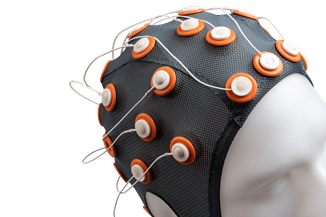
\includegraphics[width=10cm]{img/background/eeg_headcap.png}
\centering
\caption{An example of standard EEG headset}\label{fig_eeg_headcap}
\end{figure}

Standard EEG-based \ac{BCIs} usually require the subjects to wear a head-cap (Fig. \ref{fig_eeg_headcap}) with 16, 32 or 64 electrodes placed over the scalp following the standard 10-20 system . These electrodes usually require the displacing of conductive gel to obtain a stable and qualitative signal. While this type of setup is acceptable for researchers in experimental environments, it is almost impossible to imagine a daily adoption from users. This problem is nowadays partly addressed by wearable EEG-capable headsets like Emotiv Epoc, Neurosky Mindwave, Muse Headband, NextMind, Melomind (Fig. \ref{fig_melomind}.a) and many others, that mostly feature EEG capabilities with 2 up to 16 soft dry electrodes, and do not require conductive gel to capture the electric signal of the brain. While the quality of the signal is not usually as good and complete as the standard EEG-based devices, the setup of these portable \ac{BCIs} is seamless and often requires just a simple calibration making them suitable for both researchers and consumers. The experimental and analytical phases of this study have been conducted in collaboration with myBrainTechnologies, a startup based in Paris that designed Melomind to offer a real-time auditory neurofeedback application to induce a relaxation state. Apart from its designed purpose, Melomind is a fully featured \ac{BCI} that comes in two versions, standard and Q+. 

 \begin{figure}[!h]
    \centering
\subfloat[][]{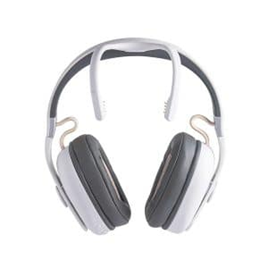
\includegraphics[width=0.4\textwidth]{img/background/fig_melomind.png}}%{1.jpeg}}
\hfil
\subfloat[][]{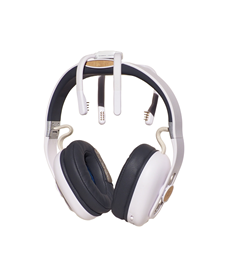
\includegraphics[width=0.4\textwidth]{img/background/fig_melomind_q+.png}}%{2.jpeg}}
    \caption{a) Melomind with 2 dry electrodes (on the flexible antennas), and 2 textile electrodes on the cushions.  \\ b) Melomind Q+ with 4 dry electrodes (on the flexible antennas), and 2 textile electrodes on the cushions.}
    \label{fig_melomind}%
    \end{figure}

The standard version used in the experiment features Bluetooth headphones with 2 textile reference electrodes and 2 dry electrodes for recording that can be placed on the parietal area in correspondence of the P3/P4 electrodes or in the frontal area in correspondence of the AF3/AF4 electrodes on the 10-20 system. The Q+ version (Fig. \ref{fig_melomind}.b) was still under development at the time of the experiment, and it is identical to the standard version except that it features 4 dry electrodes for simultaneous recording on the frontal and parietal areas, an accelerometer, and a \ac{PPG} sensor to capture heart rate. Melomind records EEG signals at a sampling rate of 250 Hz and the acquisition application uses an algorithm called \emph{QualityChecker} to help the researchers visually estimate the quality of the recorded signal in real-time. Both the EEG signals and the quality values are saved together with other metadata in a \emph{.json} file at the end of the recording. The peculiar design of Melomind allows it to play music with very good sound quality while simultaneously recording EEG signals, thus making it a good choice for experiments and applications based on auditory stimuli.

\section{A circumplex model of affect}
\label{sec:circumplex_model}
Defining what exactly is an emotion or how to measure emotions is non-trivial and has been a matter of several studies by psychologists and cognitive scientists over the last century. Many explanations and definitions have been given resulting in a wide plethora of emotional models, sometimes discordant with each other. Recently, the circumplex model of affect \cite{russell_circumplex_1980} proposed by James Russel in 1980, often referred to as the \ac{VA} model (Fig. \ref{fig_russel}), has become very popular due to its simplicity yet its efficiency in representing emotions in a 2-dimensional coordinate system. 
\begin{figure}[h!]
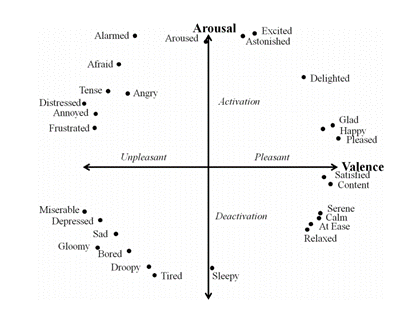
\includegraphics[width=12cm]{img/background/russel_valence_arousal.png}
\centering
\caption{Valence-Arousal model taken from J.Russell \cite{russell_circumplex_1980} }\label{fig_russel}
\end{figure}
In the \ac{VA} model, the valence of an emotion intended as a spectrum between an unpleasant and a pleasant feeling represented on the X-axis of a Cartesian coordinate system, while the arousal of emotion intended as the physiological and psychological level of activity is represented on the Y-axis of the coordinate system. In the 4 quadrants originated by the intersection of the valence and arousal axes, Russel positioned a total of 28 basic and complex emotions through an experiment involving hundreds of participants that produced a similarity matrix geometrically representing the relations between these 28 words. While the subjective perception of where emotions should be placed might differ from the model’s labelling, the VA model is still widely used because it simplifies the visualization of these emotional relations and can be easily integrated into tools for self-assessment of emotions.
Russel’s model is far from being perfect and other models tried to address some of the limitations, for example the \ac{SAM} \cite{bradley_measuring_1994} allows the self-assessment of emotions in a 3-dimensional scale defined by valence, arousal and dominance while the \ac{PANAS} \cite{watson_development_nodate} were developed to reflect the extent to which a person feels enthusiastic, active, and alert using two 10-item mood scales. However, the VA model remains a popular choice among researchers for the classification of music-elicited emotions, and, for this reason and the previously mentioned simplicity, it was chosen as main emotion self-assessment tool. Some of its limitations are also discussed in the scope of this study (see Chapter \ref{chap:discussion}).

\section{Models of emotional correlates in brain activity}
\label{sec:emotional_correlates}
The connection between music and emotions has been a matter of great interest for researchers as music has shown its great potential for evoking a wide variety of emotions. Musicians and composers intuitively know from their experience what combination of notes, chords, tempo, or pitch is likely to evoke a specific emotion and this information is valuable both in terms of artistic expression and commercial use. Correlates between emotions and the physiological effects elicited on the human body have been studied thoroughly with the intent to define a standard model for the analysis and processing of emotional information. In 2001, Schmidt and Trainor \cite{schmidt_frontal_2001} conveniently reviewed the main models for analysis of emotional valence and arousal (referred to as intensity) in the brain activity measured through EEG. The first model reviewed is from Davidson \cite{davidson_anterior_1992}, which introduced the concept of organizing emotions around approach-avoidance tendencies in the brain. According to Davidson’s model, emotions are differentially lateralized in the frontal region of the brain. In particular, the left frontal area is involved in the experience of positive emotions and the right frontal region is involved in the experience of negative emotions. The second model reviewed, brought up by Dawson \cite{dawson_frontal_1994} and Schmidt [18] states that the pattern of absolute activation in the frontal region may reflect the intensity (arousal) of the affective experience. They supported this model with numerous studies that brought data evidence of such patterns. The third model, proposed by Heller \cite{heller_neuropsychological_1993}, considers both dimensions and argues that frontal and right parietal-temporal regions are involved in the processing of emotions. According to his model, the frontal region modulates the emotional valence similarly to the model proposed by Davidson. Heller further states that the right parietal region is involved in the modulation of autonomic and behavioural arousal, higher levels of parietal-temporal activity are associated with high levels of arousal. In summary, these studies bring evidence that asymmetrical frontal EEG activity may reflect the valence of emotion experienced, while frontal and parietal absolute activation may reflect the intensity of the emotional experience. The resulting models lay the foundations for the analysis of emotions regardless of the stimulus; the application of these models to the analysis of music-elicited emotions is further discussed below (see Chapter \ref{chap:related_work}).

\section{Spectral features and emotional neuromarkers}
\label{sec:neuromarkers}
The power spectrum of the EEG signal can be classified into five main frequency bands associated to specific cognitive processes: 
\begin{itemize}
\item  	\textbf{Delta waves} (0.5hz to 3hz): associated to deepest meditation states and dreamless sleep.
\item 	\textbf{Theta Waves} (3hz to 8hz): associated to learning, working memory and intuition.
\item 	\textbf{Alpha Waves} (8hz to 12hz): the most prominent in brain activity, it is associated with the resting state of the brain, with coordination and alertness.
\item 	\textbf{Beta Waves} (12hz to 33hz): another commonly found wave in the brain activity, it is associated with active cognitive tasks, attention, and movement.
\item 	\textbf{Gamma Waves} (25hz to 100h): associated to high level cognitive processing tasks, senses, and perceptions.
\end{itemize}
For this study, the most sensitive frequency bands for the study of emotions, according to literature, were considered: Theta, Alpha and Beta. These frequency bands have been often encountered in the analysis of music-elicited emotions and used in the \ac{ER} task. The approach of this study was to calculate bio-markers from the brain activity, referred to as “neuromarkers”, to represent differential and rational measurements supported by the models of emotional correlates. These neuromarkers are a convenient mathematical expression of the theories of frontal asymmetrical activity and regional absolute activation in the brain activity, and some equivalent version can be found in the related studies with similar or different names. The computed neuromarkers are the following:
	
\begin{itemize}
\item \textbf{\ac{AWI}}: asymmetry index representing the approach-avoidance tendencies of Alpha waves in the frontal area of the brain and computed as difference of Alpha power between the two frontal electrodes after normalization against the baseline using the following formula 
		\[AW = (Pow_\alpha AF4 - Pow_\alpha AF3) \]
\item \textbf{\ac{FMTI}}: index representing absolute increasing/decreasing activation in the Theta activity on the Fz channel compared to the baseline period, it is inferred between the frontal electrodes after normalization against the baseline using the following formula 
			\[FMT = Mean(Pow_\theta AF4 , Pow_\theta AF3)  \]
\item \textbf{\ac{SASI}}: index representing the balance of Theta and Beta frequency band power, computed on both frontal electrodes after normalization against the baseline using the following formula 
		\[SASI(AF3)= \frac{(Pow_\beta AF3 - Pow_\theta AF3)}{(Pow_\beta AF3 + Pow_\theta AF3)} \] \[SASI(AF4)= \frac{(Pow_\beta AF4 - Pow_\theta AF4)}{(Pow_\beta AF4 + Pow_\theta AF4)} \]  
\end{itemize}

\ac{AWI} and \ac{SASI}, or equivalent measurements, have been reported to reflect the emotional valence \cite{schmidt_frontal_2001,orgo_effect_2015}. \ac{FMTI}, or equivalent measurements, has been reported to reflect the level of appreciation \cite{sammler_music_nodate}, the emotional valence \cite{reuderink_valence_2013} and the arousal dimension of emotions (arousal) \cite{zhao_frontal_2018}. A multitude of reviewed studies \cite{lin_eeg-based_2009,lin_eeg-based_2010}, \cite{wu_estimation_2017,thammasan_continuous_2016}, \cite{ koelstra_deap_2012} (see Chapter \ref{chap:related_work}) make use of equivalent measurements as features for classification emotional valence and arousal. Zhao et al. \cite{zhao_frontal_2018} investigated the use of asymmetries and mid-line absolute power in the Theta, Alpha and Beta frequency bands to classify discrete emotion within the same emotional spectrum and were able to successfully classify four emotions with appreciable precision. To strengthen the effectiveness in the classification of emotional valence and arousal, the neuromarkers were supported by an extra set of features of the \ac{EEG} signal, extracted in the same frequency bands of interest: raw power, skewness, kurtosis, standard deviation, ratio, and relative spectral difference (see Chapter \ref{chap:methods}).

